\documentclass[11pt,a4paper]{book}
\usepackage[english,greek]{babel}
\usepackage[utf8x]{inputenc}
\usepackage[noend]{algpseudocode}
\usepackage{algorithm}
\usepackage{amssymb,latexsym,amsmath,ucs,amsthm,setspace,graphicx,fancyvrb,float}
\usepackage{hyperref}
\usepackage{tkz-graph}
\usepackage{subfig}
\newtheorem*{lemma}{Λήμμα}
\newcommand{\HRule}{\rule{\linewidth}{0.5mm}}
\newcommand{\defeq}{\overset{\underset{\mathrm{def}}{}}{=}}
\makeatletter
\DeclareMathOperator*{\argmin}{arg\,min}
\makeatother
\raggedbottom
\begin{document}

\begin{titlepage}
\begin{center}


\includegraphics[width=0.15\textwidth]{Pyrforos3.png}\\[1cm]
\textsc{\LARGE Εθνικό Μετσόβιο Πολυτεχνείο}\\[1.5cm]

\Large{ 3η Γραπτή Άσκηση }\\[0.5cm]

% Title
\begin{doublespace}
\HRule \\[0.4cm]
{\huge \bfseries
Αλγόριθμοι \& Πολυπλοκότητα
}\\[0.4cm]
\end{doublespace}

\HRule \\[1.5cm]

\begin{minipage}{0.4\textwidth}
\begin{flushleft} \large
\emph{Σπουδαστής:} \\
Διονύσης \textsc{Ζήνδρος} (06601)\\
\textlatin{\textless dionyziz@gmail.com\textgreater}
\end{flushleft}
\end{minipage}
\begin{minipage}{0.4\textwidth}
\begin{flushright} \large
\emph{Διδάσκοντες:} \\
Στάθης \textsc{Ζάχος}\\
Δημήτρης \textsc{Φωτάκης}
\end{flushright}
\end{minipage}

\vfill

{\large 24 Ιανουαρίου 2011}
\end{center}
\end{titlepage}

\section*{Άσκηση 1}
Για να ελέγξουμε αν ο γράφος είναι διμερής, χρωματίζουμε μία ακμή αυθαίρετα και στη συνέχεια για κάθε χρωματισμένη ακμή χρωματίζουμε τους γείτονές της με το αντίθετο χρώμα έως ότου ολοκληρωθεί η διαδικασία ή καταλήξουμε σε αντίφαση.

\selectlanguage{english}
\begin{algorithm}[H]
\caption{\textgreek{Άσκηση 1}}
\begin{algorithmic}[1]

\Procedure{Bipartite}{$V, E$}
    \For {$v \in V$}
        \State $color[ v ] \gets \emptyset$
    \EndFor
    \State $q \gets \{ V[ 0 ] \}$
    \State $color[ V[ 0 ] ] \gets \top$
    \While {$q \neq \emptyset$}
        \State $s \gets \textlatin{remove and return an element of q}$
        \State $paint \gets \lnot color[ s ]$
        \For {$\text{neighbour } t \text{ of } s$}
            \If {$color[ t ] \neq \emptyset$}
                \If {$color[ t ] \neq paint$}
                    \State \Return $\bot$
                \EndIf
            \Else
                \State $color[ t ] \gets paint$
                \State $q \gets q \cup \{ t \}$
            \EndIf
        \EndFor
    \EndWhile
    \State \Return $\top$
\EndProcedure
\end{algorithmic}
\end{algorithm}
\selectlanguage{greek}

\section*{Άσκηση 2}
Διασχίζουμε το γράφο χρησιμοποιώντας \textlatin{BFS} και διατηρούμε κάθε φορά το πλήθος των τρόπων με τους οποίους φτάσαμε σε κάθε κόμβο.

\selectlanguage{english}
\begin{algorithm}[H]
\caption{\textgreek{Άσκηση 2}}
\begin{algorithmic}[1]

\Procedure{ShortestCount}{$V, E, s, t$}
    \For {$v \in V$}
        \State $visited[ v ] \gets 0$
        \State $distance[ v ] \gets \infty$
    \EndFor
    \State $visited[ s ] \gets 1$
    \State $distance[ s ] \gets 0$
    \State $q \gets \Call{EmptyQueue}$
    \State $\Call{Push}{q, s}$
    \While{$\lnot \Call{Empty}{q}$}
        \State $u \gets \Call{Pop}{q}$
        \If{$u = t$}
            \State \Return $visited[ t ]$
        \EndIf
        \For {$\text{neighbour } v \text{ of } u$}
            \If {$distance[ v ] = \infty$}
                \State $\Call{Push}{q, u}$
            \EndIf
            \If {$distance[ u ] + 1 \leq distance[ v ]$}
                \State $distance[ v ] \gets distance[ u ] + 1$
                \State $visited[ v ] \gets visited[ v ] + visited[ u ]$
            \EndIf
        \EndFor
    \EndWhile
\EndProcedure
\end{algorithmic}
\end{algorithm}
\selectlanguage{greek}

\section*{Άσκηση 3}
\subsection*{(α)}
Ο γράφος της άσκησης 4 με $L = \{ C \}$ είναι ένα παράδειγμα γράφου που έχει διαφορετικό ΕΣΔ υπό περιορισμούς.

\subsection*{(β)}
\selectlanguage{english}
\begin{algorithm}[H]
\caption{\textgreek{Άσκηση 3}}
\begin{algorithmic}[1]

\Procedure{ConstraintedMST}{$V, E, L$}
	\If {$|V| \leq 2$}
	    \State \Return $E$
	\EndIf
    \For {$v \in V$}
        \State $adj[ v ] \gets \emptyset$
        \State $best[ v ] \gets \infty$
    \EndFor
    \For {$e = (u, v, w) \in E$}
    	\If {$u \in L \oplus v \in L$}
	    	\For {$s \in \{u, v\}$}
		        \If {$s \in L$}
    		        \If {$w < best[ s ]$}
            		    \State $best[ s ] \gets w$
        	    	    \State $adj[ s ] \gets \{ e \}$
	    	        \EndIf
    	        \EndIf
        	\EndFor
        \Else
            \State $adj[ v ] \gets adj[ v ] \cup \{ e \}$
        \EndIf
    \EndFor
    \State \Return $\Call{Prim}{V, adj}$
\EndProcedure
\end{algorithmic}
\end{algorithm}
\selectlanguage{greek}

\section*{Άσκηση 4}
\subsection*{(α)}

Ο ακόλουθος γράφος έχει μοναδικό ΕΣΔ, αλλά περιέχει ακμές ίδιου βάρους:

\selectlanguage{english}
\begin{figure}[ht]
	\centering
		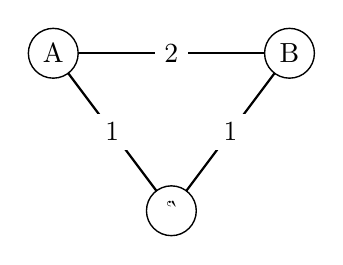
\begin{tikzpicture}
			\Vertex[x=0,y=0,L=A]{1}
			\Vertex[x=3,y=0,L=B]{2}
			\Vertex[x=1.5,y=-2,L=C]{3}

			\Edge[label=2](1)(2)
			\Edge[label=1](1)(3)
			\Edge[label=1](2)(3)
		\end{tikzpicture}
\end{figure}
\selectlanguage{greek}

\subsection*{(β)}
Ο γράφος του υποερωτήματος (α) έχει μοναδικό ΕΣΔ αλλά περιέχει ακμές ίδιου βάρους που είναι οι ελάχιστες που διασχίζουν την ίδια τομή.

\begin{lemma}
Κάθε ακμή ενός ΕΣΔ ενός συνεκτικού μη κατευθυνόμενου ζυγισμένου γράφου είναι η ελάχιστη που διασχίζει κάποιο κόψιμο.
\end{lemma}
\begin{proof}
Έστω τέτοιος γράφος $G = (V, E, w)$ με ένα ΕΣΔ του $T \subseteq E$ και έστω ότι υπάρχει κάποια ακμή $e = (u, v) \in T$ τέτοια ώστε να μην υπάρχει κόψιμο του G το οποίο να είναι η ελάχιστη που το διασχίζει. Τότε έστω $K$ το ΕΣΔ που κατασκευάζει ο αλγόριθμος του \textlatin{Kruskal}. Κατά την εκτέλεση του αλγορίθμου, υπάρχει κάποιο βήμα κατά το οποίο γίνεται ένωση των ανεξάρτητων συνόλων που περιέχουν τους κόμβους $u$ και $v$ μέσω κάποιας ακμής $f$ η οποία είναι ελάχιστη σε ένα κόψιμο το οποίο διασχίζει και η $e$ και άρα $w(f) < w(e)$. Όμως στο $T$ η ακμή $e$ μπορεί να αντικατασταθεί από την $f$ και το δέντρο να παραμείνει συνεκτικό και με βάρος $w( T \cup \{f\} \setminus \{e\}) < w( T )$. Άρα το $T$ δεν είναι ΕΣΔ, κάτι το οποίο αποτελεί αντίφαση.
\end{proof}

\begin{lemma}
Κάθε συνεκτικός μη κατευθυνόμενος ζυγισμένος γράφος στον οποίο για κάθε τομή η ακμή ελάχιστου βάρους που τη διασχίζει είναι μοναδική έχει μοναδικό ΕΣΔ.
\end{lemma}
\begin{proof}
Έστω τέτοιος γράφος $G = (V, E, w)$ και δύο ΕΣΔ του, $T \subseteq E$ και $T' \subseteq E$,
με $T \neq T'$ και $w(T) = w(T')$.

Τότε, επειδή $T \neq T$, θα υπάρχει κάποια ακμή $e = (u, v)$ με $e \in T \land e \not\in T'$. Από το παραπάνω λήμμα, η $e$ θα είναι η ελάχιστη που διασχίζει κάποιο κόψιμο του $T$, έστω $S$.

Τώρα, επειδή το $T'$ είναι συνεκτικό δέντρο, θα υπάρχει μοναδικό μονοπάτι από τον κόμβο $u$ στον κόμβο $v$ που διασχίζει το $S$ με κάποια ακμή, έστω $e' \neq e$. Αφού $w(e) < w(e')$, αντικαθιστώντας την ακμή $e'$ με την $e$ στο $T'$ παίρνουμε ένα συνεκτικό δέντρο με βάρος $w(T' \cup\{e\} \setminus \{e'\}) < w(T')$. Άρα το $T'$ δεν είναι ελάχιστο συνεκτικό δέντρο, κάτι το οποίο αποτελεί αντίφαση.

Άρα το ΕΣΔ είναι μοναδικό.
\end{proof}

\subsection*{(γ)}
\begin{lemma}
Το ΕΣΔ ενός συνεκτικού ζυγισμένου μη κατευθυνόμενου γράφου είναι μοναδικό ανν κάθε ακμή του είναι η μοναδική ελάχιστη σε κάποιο κόψιμο του γράφου.
\end{lemma}

\begin{proof}
Έστω $G = (V, E, w)$ ένας τέτοιος γράφος και έστω $K$ ένα ΕΣΔ του.

Θα δείξουμε ότι αν κάθε ακμή του $K$ είναι η μοναδική ελάχιστη σε κάποιο κόψιμο, τότε το δέντρο είναι μοναδικό. Πράγματι, έστω ότι υπάρχει ΕΣΔ $T \neq K$. Τότε θα υπάρχει ακμή $e = (u, v) \in K \land e \not\in T$. Από την υπόθεση, υπάρχει κόψιμο $S$ το οποίο η $e$ διασχίζει ως μοναδική ελάχιστη. Επειδή το $T$ είναι συνδετικό, θα υπάρχει μοναδικό μονοπάτι που συνδέει τους κόμβους $u$ και $v$ το οποίο διασχίζει το κόψιμο $S$ χρησιμοποιώντας κάποια ακμή $f \neq e$. Επειδή η $e$ είναι ελάχιστη, θα είναι $w(e) < w(f)$. Αντικαθιστώντας την $f$ με την $e$ στο $T$ προκύπτει ΕΣΔ με $w( T \cup \{ e \} \setminus \{ f \} ) < w( T )$ κάτι το οποίο αποτελεί αντίφαση. Άρα το $K$ είναι μοναδικό.

Αντίστροφα, έστω ότι το $K$ είναι μοναδικό. Τότε ο αλγόριθμος του \textlatin{Kruskal} θα δώσει το $K$. Έστω, τώρα, ότι υπάρχει κάποια ακμή $e \in K$ που δεν είναι ελάχιστη σε κανένα κόψιμο του $G$. Τότε ο αλγόριθμος δεν θα μπορούσε να την έχει επιλέξει ποτέ, και άρα $e \not\in K$. Αυτό αποτελεί αντίφαση, και άρα όλες οι ακμές είναι ελάχιστες σε κάποιο κόψιμο.
\end{proof}

\subsection*{(δ)}

\section*{Άσκηση 5}
\subsection*{(α)}
\begin{lemma}
Σε ένα συνεκτικό κατευθυνόμενο ζυγισμένο γράφο, για κάθε κύκλο υπάρχει ΕΣΔ που δεν περιέχει την ακμή μέγιστου βάρους του κύκλου αυτού.
\end{lemma}

\begin{proof}
Έστω τέτοιος γράφος $G = (V, E, w)$ με κάποιον κύκλο $C$ και έστω ένα ΕΣΔ $T \subseteq E$ που περιέχει την ακμή $e$ μέγιστου βάρους του $C$. Τότε έστω το δάσος $T \setminus \{ e \}$ που θα αποτελείται από δύο συνδεδεμένους υπογράφους. Θα υπάρχει μία ακμή $f \in E$ που θα συνδέει αυτούς τους δύο συνδεδεμένους υπογράφους με $f \neq e$ και άρα $w( f ) \leq w( e )$. Αντικαθιστώντας την $e$ με την $f$ στο $T$ προκύπτει ένα συνεκτικό δέντρο με βάρος $w( T \cup \{ f \} \setminus \{ e \} ) \leq w( T )$. Άρα το $T \cup \{ f \} \setminus \{ e \}$ είναι ΕΣΔ.
\end{proof}

\subsection*{(β)}
\begin{lemma}
Ο αντίστροφος αλγόριθμος του \textlatin{Kruskal} είναι ορθός.
\end{lemma}

\begin{proof}
Σε κάθε βήμα $i$, ο αλγόριθμος διατηρεί τον ελάχιστου κόστους συνδετικό υπόγραφο $G_i$ με ακριβώς $j(i) = m - i + 1$ ακμές. Πράγματι, στο $1$ο βήμα, ο υπόγραφος είναι ίσος με τον αρχικό γράφο και άρα συνδετικός και ελάχιστος. Έστω ότι ο υπόγραφος είναι συνδετικός και ελάχιστος στο $i$-οστό βήμα. Τότε έστω $e = (u, v)$ η επόμενη ακμή που θα επιλεγεί.

Στην περίπτωση που η $e$ είναι γέφυρα του $G_i$ ανάμεσα σε δύο συνδεδεμένα τμήματα $C_1$ και $C_2$, δηλαδή διασχίζει το κόψιμο $S = ( C_1, C_2 )$ του αρχικού γράφου, η ακμή αυτή δε θα λείπει από κανέναν ελάχιστο συνδετικό υπογράφο $G_k$ με $k > i$. Αυτό φαίνεται ως εξής. Έστω ότι η $e$ έλειπε από τον $G_k$· τότε αυτός θα περιείχε κάποια ακμή $f \neq e$ που διασχίζει το $S$ για να είναι συνδεδεμένος. Όμως θα είναι $w(f) > w(e)$ διότι, λόγω άπληστης ιδιότητας, η $f$ είχε αφαιρεθεί πριν το $i$-οστό βήμα αφού η $e$ ήταν γέφυρα του $G_i$. Αντικαθιστώντας την $f$ με την $e$ λαμβάνουμε ένα συνδετικό υπόγραφο ίδιου πλήθος ακμών με βάρος $w( G_k \cup \{ e \} \setminus \{ f \} ) < w( G_k )$. Άρα το $G_k$ δεν θα ήταν ελάχιστο χωρίς την ύπαρξη της $e$. Συνεπώς μπορούμε με ασφάλεια να διατηρήσουμε την $e$ στον υπογράφο και να προχωρήσουμε στην επόμενη ακμή στο ίδιο βήμα.

Στην περίπτωση που η $e$ δεν είναι γέφυρα του $G_i$ τότε ανήκει σε ένα κύκλο του $G_i$. Εργαζόμενοι παρόμοια όπως στο παραπάνω θεώρημα, είναι εμφανές ότι η $e$ δεν ανήκει στον υπόγραφο $G_{i+1}$. Την αφαιρούμε, λοιπόν, και προχωράμε στο επόμενο βήμα.

Χρησιμοποιώντας, τώρα, τη μαθηματική επαγωγή, έχουμε αποδείξει την αμετάβλητη ιδιότητα της επανάληψης. Τέλος, ο ελάχιστος συνδετικός υπόγραφος με ακριβώς $n - 1$ είναι ΕΣΔ.
\end{proof}

\subsection*{(γ)}

\end{document}
